\documentclass[12pt, a4paper, oneside]{article}

\usepackage[margin=1.5cm]{geometry}
\usepackage{fancyhdr}
\usepackage{graphicx}
\usepackage[compact]{titlesec}
\usepackage{enumitem}
\usepackage{amssymb}
\usepackage{url}
\usepackage{float}
\usepackage[labelfont=bf]{caption}

\pagestyle{fancy}
\fancyhf{}
\lhead{CS324 Report}
\chead{\thepage}
\rhead{u1919771}

\setlength{\parskip}{0.5cm}
\renewcommand{\baselinestretch}{1.2}

\graphicspath{{./img/}}

\begin{document}
    \LARGE
    \begin{center}
        \textbf{CS324 Coursework Supporting Document}
    \end{center}

    \normalsize
    \flushleft

    \section{Overview}

    \textbf{Home Sweet Home} is a simple parkour game developed in \textit{WebGL2} using \textit{THREE.js} \cite{three} as a rendering engine and \textit{CANNON-es} \cite{cannon-es} as a physics engine; it was orinally inspired by a \textit{THREE.js} demo program \cite{original_inspiration}. The game is run in a web browser programmed using Javascript, with the addition of game menu written in HTML5 and CSS3. \textit{JQuery} \cite{jquery} is also used as a supplementary library to facilitate manipulation of HTML document objects such as handling event listeners.

    \begin{figure}[H]
        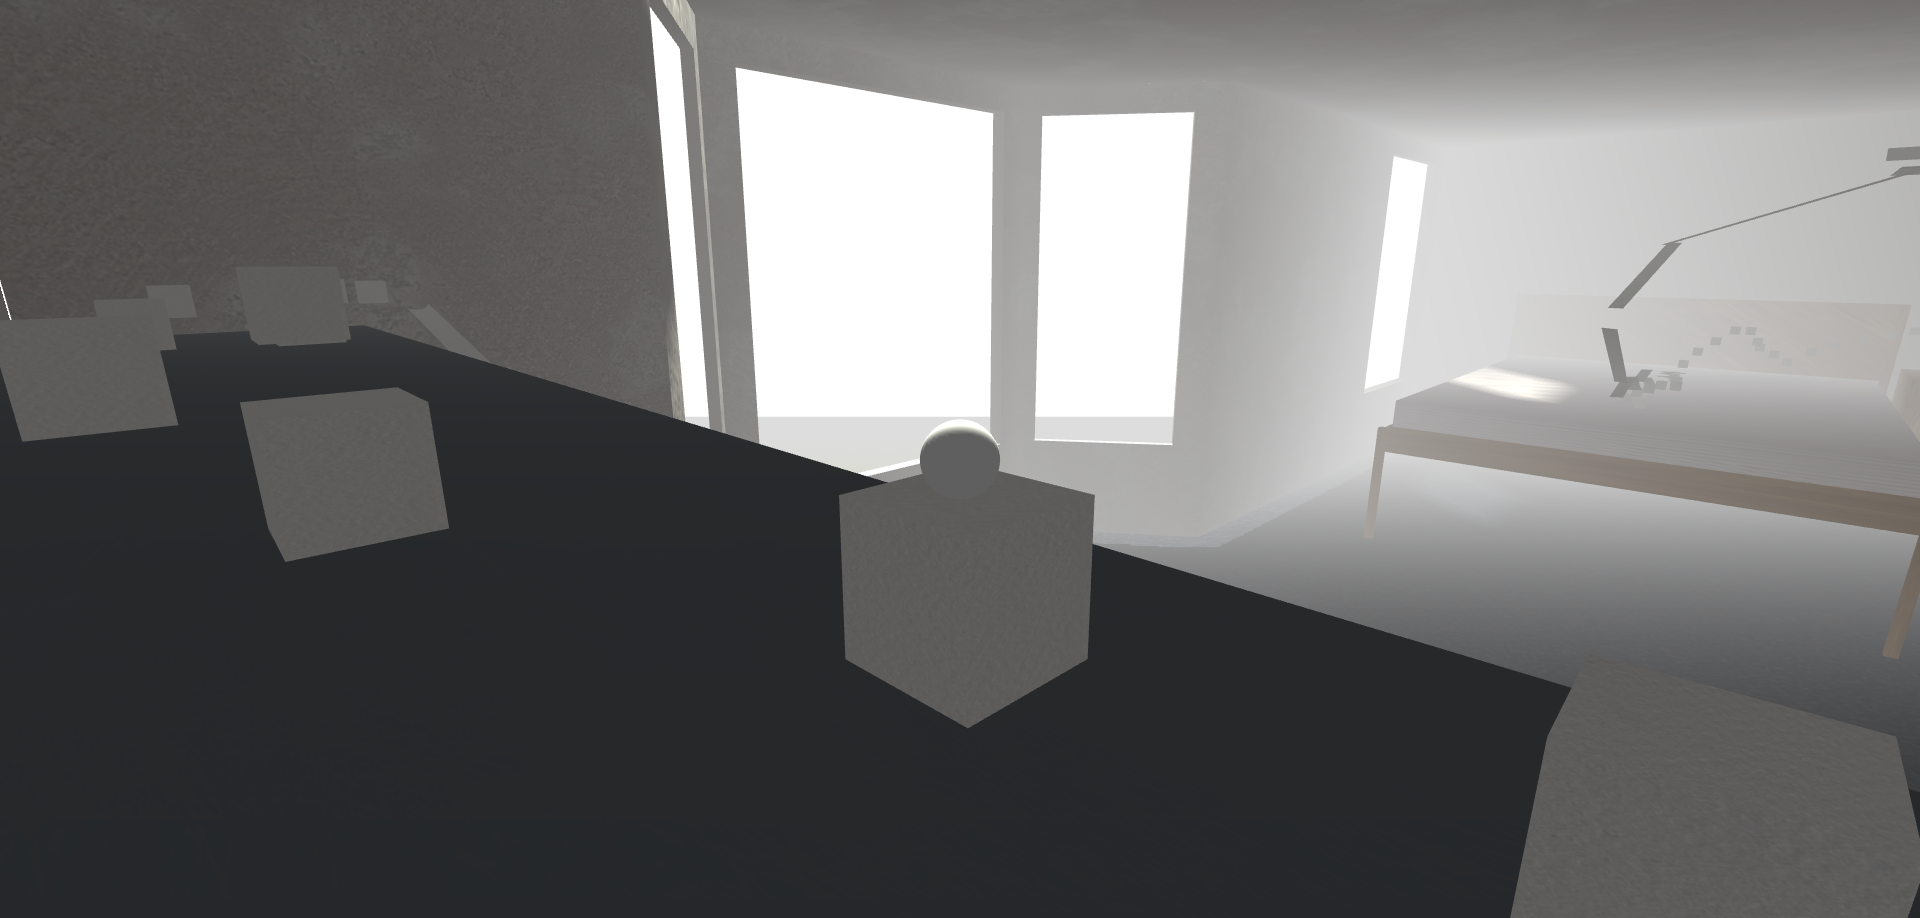
\includegraphics[width=\textwidth]{showcase.png}
        \caption{A showcase of an in-game screenshot.}
    \end{figure}

    \section{The Game}

    In the game, the player will be controlling a sphere as the main character, navigating around a house with nearly 1:1 scale of a real-life bedroom \footnote{In fact, it is my bedroom.}. The main game map, the bedroom, is modelled using \textit{Blender} and exported as \textit{glb} format; texture used in the map is gathered online \cite{texture_res} with permission to use for individual project.

    \subsection{Features}

    The original \textit{THREE.js} program uses ray casting for collision detection and only detects collision at player's foot. With the help of \textit{CANNON-es}, more accurate physics can be simulated including gravity and friction.
    
    House model and various game objects are imported using \textit{GLTFLoader} provided by \textit{THREE.js}. To construct correct axis-aligned bounding box for collision detection, each individual shape in the model such as furnitures around the house and obstacles, needs to have its bounding box computed and transform the the coordinate system from model to world space.

    The character controller is modified from a demo program shown in \textit{CANNON-es} \cite{cannon_controller}. In particular, the character controller has support to momentum, which allows the character to move by a short distance when it is stopping. Certain obstacles are relatively farther away such that player should maintain an initial velocity to increase the jumping distance to land on the target. Additionally, the camera allows cycling view between first-person and second-person \footnote{It (as well as top-down view) may also be referred as third-person.}. The second-person view is achieved by displacing the camera along its negated view direction by a certain distance.

    The game also features death system to avoid cheating or allow player to restart. When the character collides with any surface, the game reads the altitude of the surface the character was previouly stayed on, and calculate the delta altitude. If the character has fallen by greater than a limit, a death screen will be displayed and allows the player to restart the level.

    \begin{figure}[H]
        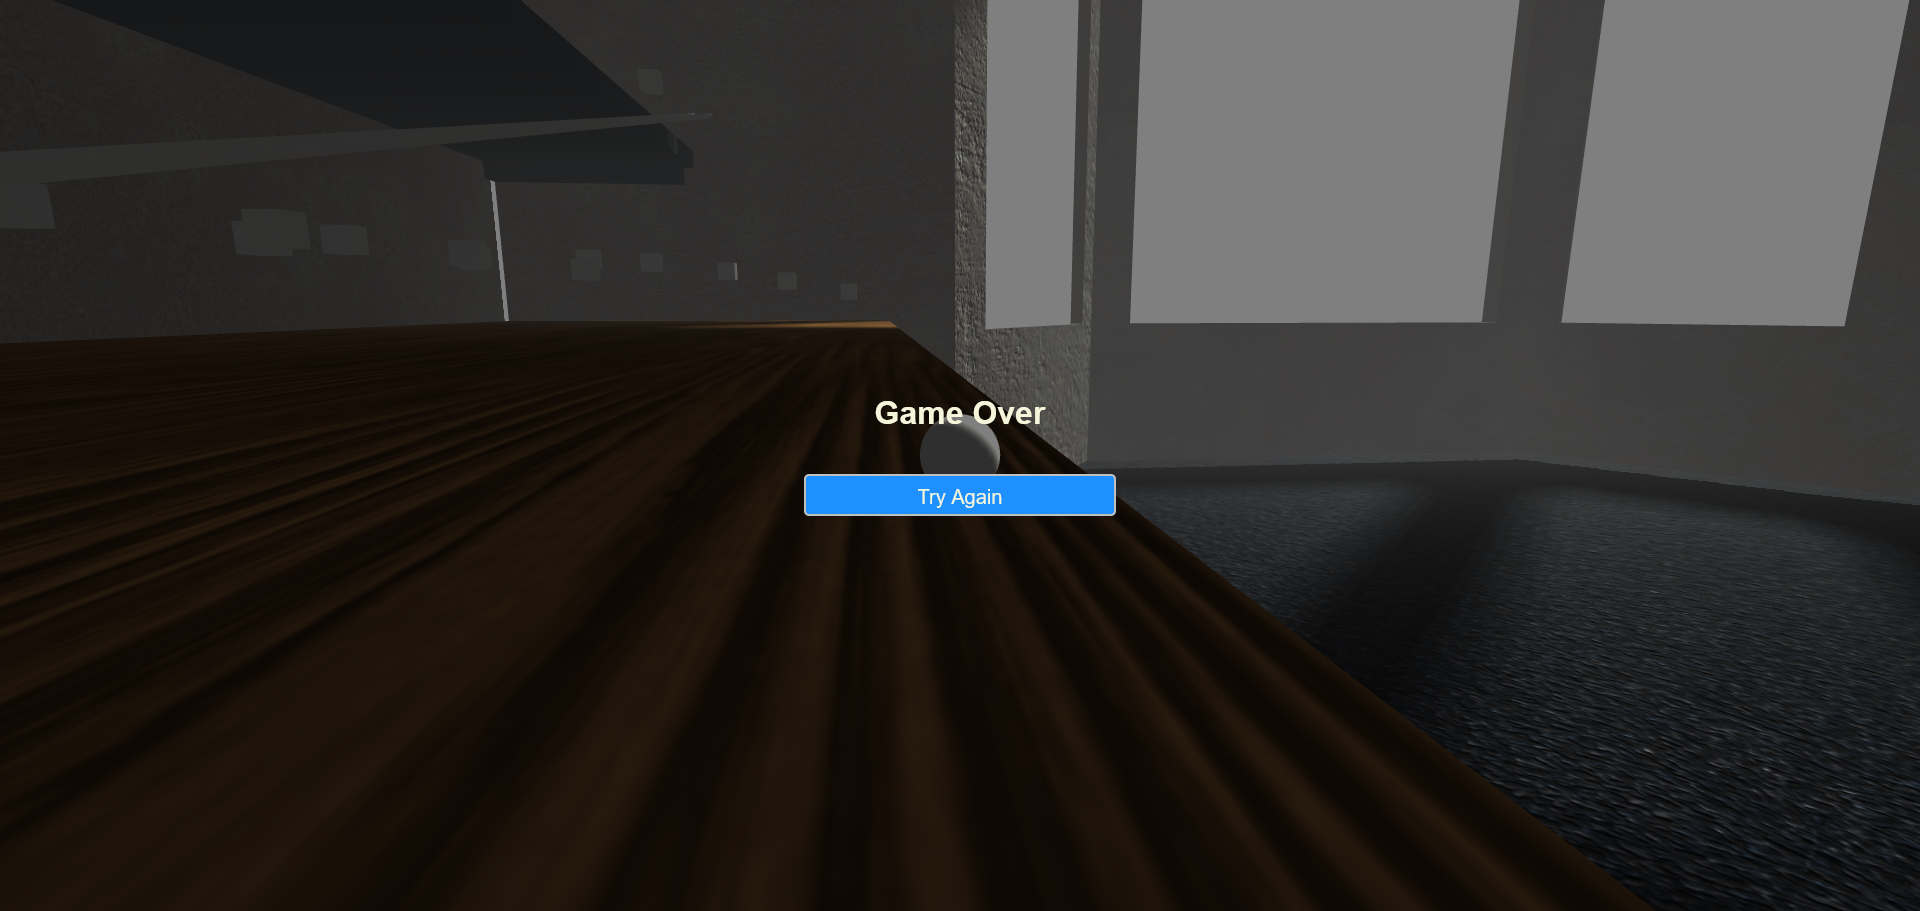
\includegraphics[width=\textwidth]{death.png}
        \caption{Demonstrates a death screen when the player is attempting to jump from very high aboved.}
    \end{figure}

    At the end of each level, there is a \textit{ghost} collision object which by default is invisible and does not produce any collision force, instead it triggers a collision event for the system to check if the character has reached the goal, and progress the player to, either the next level or the end of game if there is no more level left.

    \begin{figure}[H]
        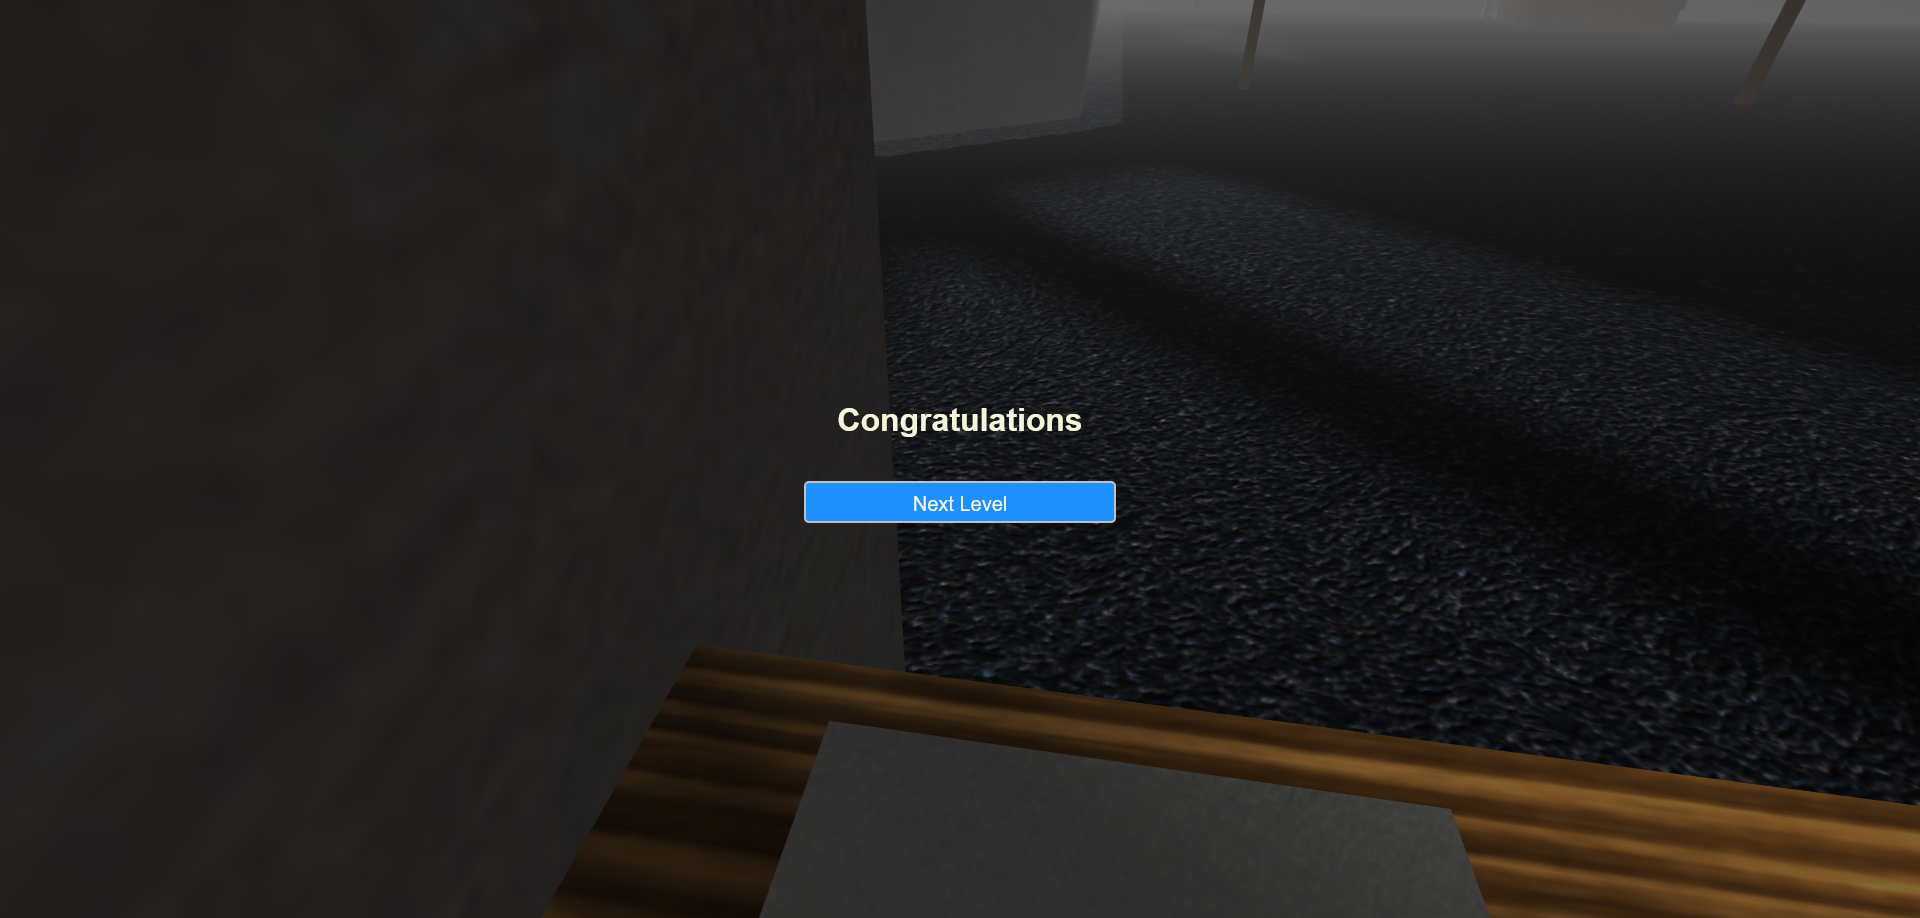
\includegraphics[width=\textwidth]{progress.png}
        \caption{Illustrates the game progression screen when the player passes the current level.}
    \end{figure}

    \subsection{Designs}

    \subsubsection{Rendering}

    Rendering is done purely using \textit{THREE.js}. There are two light sources in the game, one being the sun light outside the house and the other being the ceiling light in the room. Both lights cast shadows; shadow is handled using variance shadow mapping. Compared to percentage closed filtered shadow, it allows softer shadow edges and is cheaper to compute. Shadow maps have resolution of 1024x1024.

    Texture is used in all objects in the scene except the character-controlled sphere. All such objects have at least albedo and normal maps, and some objects have also roughness and ambient-occlusion maps applied. Textures are repeat-wrapped with OpenGL-generated mipmapping, and linear, x16 anisotropy filtered.

    The scene is rendered with fog to make sure the player cannot see the camera far clipping plane. The framebuffer has x8 multi-sampling anti-aliasing turned on.

    \subsubsection{Map}

    The bedroom is modelled using \textit{Blender}.

    \subsubsection{Levels}

    The game contains 2 independent levels.
    
    \section{Limitations and Future Works}

    \begin{itemize}[label=\(\diamond\)]
        \item Collision detection for the house wall is disabled as significant amount of the time is needed to construct a collision mesh for a non-convex shape in real-time. Improvement can be made in the future such as reducing the complexity of the wall model by eliminating unnecessary vertices.
        \item Game can be exploited such that some obstacles can be bypassed.
    \end{itemize}

    \bibliographystyle{unsrt}
    \bibliography{reference}

\end{document}